\documentclass[11pt,twocolumn]{article}

% --- Codificación y lenguaje ---
\usepackage[T1]{fontenc}
\usepackage[utf8]{inputenc}
\usepackage[spanish]{babel}

% --- Matemática y fuentes ---
\usepackage{amsfonts, amssymb, amsthm}
\usepackage{derivative}
\usepackage{physics} 

% --- Gráficos y tablas ---
\usepackage{graphicx}
\usepackage{caption}        % <-- primero caption
\usepackage{subcaption}     % <-- luego subcaption
\usepackage{booktabs}

% --- Varios útiles ---
\usepackage[margin=2cm]{geometry}
\raggedbottom
\usepackage{enumitem}
\usepackage{csquotes}
\usepackage{cuted}          % para elementos a dos columnas (opcional)
\usepackage{stackrel}
% \usepackage{microtype}      % desactivado: evita el warning \showhyphens en Overleaf
\usepackage{float}
\usepackage{placeins}
% \usepackage{nameref}      % NO necesario: hyperref ya define \nameref
\usepackage[dvipsnames]{xcolor}
\usepackage{tikz}
\usetikzlibrary{calc}

% --- Bibliografía (BibTeX + apacite) ---
\usepackage[backend=biber,style=apa,language=spanish]{biblatex}
\addbibresource{referencias.bib} % tu archivo original con @online


% --- Hipervínculos (casi al final) ---
\usepackage[
  colorlinks=true,
  linkcolor=black, urlcolor=black, citecolor=black, filecolor=black,
  pdfborder={0 0 0}
]{hyperref}
% --- Colores para hipervínculos (citas en azul) ---
\hypersetup{
  colorlinks=true,
  linkcolor=black,      % refs, índice
  urlcolor=Blue,
  citecolor=Blue   % color del link de la cita
}

% --- Forzar que TODA la cita (no solo el link) salga en color
\makeatletter
\let\orig@cite\cite
\renewcommand{\cite}[1]{\textcolor{Blue}{\orig@cite{#1}}}

% Si en el texto usaste \citeA (cita textual tipo Autor (Año)),
% la convertimos también a formato entre paréntesis y color:
% --- Citas parentéticas y en color, compatible con apacite o biblatex ---
\makeatletter
% ¿Existe \citeA (apacite)? Si no, asumimos biblatex.
\@ifundefined{citeA}{%
  % --------- rama biblatex ---------
  % Si existe \parencite, la coloreamos y mapeamos \cite / \citeA a paréntesis:
  \@ifundefined{parencite}{}{%
    \let\orig@parencite\parencite
    \renewcommand{\parencite}[1]{\textcolor{Blue}{\orig@parencite{#1}}}
    \renewcommand{\cite}[1]{\parencite{#1}}      % \cite -> (Autor, Año)
    \providecommand{\citeA}[1]{\parencite{#1}}   % por si quedó \citeA en el texto
    % (Opcional) forzar \textcite también a parentético:
    % \let\orig@textcite\textcite
    % \renewcommand{\textcite}[1]{\parencite{#1}}
  }%
}{%
  % --------- rama apacite ---------
  \let\orig@cite\cite
  \renewcommand{\cite}[1]{\textcolor{Blue}{\orig@cite{#1}}} % color a (Autor, Año)
  % Hacer que \citeA (Autor (Año)) también salga parentético y en color:
  \let\orig@citeA\citeA
  \renewcommand{\citeA}[1]{\textcolor{Blue}{\orig@cite{#1}}}
}
\makeatother


\begin{document}

\begin{tikzpicture}[remember picture,overlay]
  \node[anchor=north east, inner sep=0pt]
    at ($(current page.north east)+(-1.8cm,-1.2cm)$)
    {
\includegraphics[height=2.8cm]{images/figures/UdeC_logo_azul.png}};
\end{tikzpicture}

\begin{strip}
\begin{center}
\vspace*{-5\baselineskip}
{\Large \textbf{Universidad de Concepción}}\\[-2pt]
\small Facultad de Ciencias Físicas y Matemáticas\\[-2pt]
\small \textit{Laboratorio II (510352-1)}\\[4pt]

{\Large \bfseries Informe 3: Indice de refracción de la luz }\\[2pt]
{\Large \bfseries y ley de Snell}\\
[2pt]
\small Profesor: Paulraj Manidurai\\[-2pt]
\small F. Contreras M., J. Rosas S., J. Chandia V., M. Díaz S., M. Fierro S.\\[-2pt]
\small Concepción, Chile — 5 de octubre de 2025
\end{center}
\vspace{0.5\baselineskip}
\hrule
\vspace{0.8\baselineskip}

\begin{abstract}
El presente estudio analiza el comportamiento de la luz al atravesar distintos medios con diferente densidad óptica, utilizando un montaje semicircular que permite medir con precisión los ángulos de incidencia y refracción. Se trabajó con tres materiales: acrílico, agua y una solución de agua con café, a fin de comparar la desviación del haz en medios transparentes y semitransparentes. Mediante el registro de los pares $(\theta_{1}, \theta_{2})$, se verificó la Ley de Snell y se estimó el índice de refracción de cada medio. Además, se identificó el ángulo crítico asociado a la reflexión total interna, proporcionando una base experimental para el estudio de la óptica geométrica.
\end{abstract}


\noindent\rule{\textwidth}{0.4pt}\par\vspace{0.3cm}
\end{strip}

\section{Objetivos.}

\begin{itemize}
    \item Determinar el índice de refracción de medios transparentes y semitransparentes, específicamente acrílico, agua y agua con café.
    \item Verificar experimentalmente la Ley de Snell mediante la comparación entre los valores de $\sin\theta_{1}$ y $\sin\theta_{2}$ obtenidos en cada medio estudiado.
    \item Identificar el ángulo crítico y el inicio de la reflexión total interna en medios ópticamente densos.
\end{itemize}

\section{Introducción.}

El estudio de la refracción luminosa es fundamental para comprender el comportamiento de la luz en diferentes medios y constituye la base de múltiples aplicaciones ópticas, tales como lentes, prismas y fibras de transmisión \cite{hecht_optics_2016}. Cuando un haz luminoso atraviesa una interfase entre materiales con distinta densidad óptica, su trayectoria sufre una desviación gobernada por leyes geométricas que permiten caracterizar cuantitativamente el medio mediante su índice de refracción \cite{serway_physics_2013}.

En este experimento se analiza el paso de la luz a través de medios transparentes y parcialmente turbios, utilizando configuraciones semicirculares que permiten minimizar errores de alineación y medir directamente los ángulos de incidencia y refracción. A partir de estas mediciones se busca verificar la validez de la Ley de Snell y estimar el índice de refracción de materiales como acrílico, agua y mezclas acuosas con partículas en suspensión.

Además, se aborda el fenómeno de la reflexión total interna, observable cuando la luz intenta pasar desde un medio más denso a uno menos denso. La identificación experimental del ángulo crítico constituye un método alternativo para determinar propiedades ópticas del material y permite contrastar resultados obtenidos por vías geométricas \cite{feynman_lectures_2010}. El trabajo experimental integra así fundamentos de la óptica geométrica con la caracterización cuantitativa de medios, contribuyendo a la comprensión de fenómenos de propagación y confinamiento de la luz.

\section{Marco teórico}

\subsection{Propagación de la luz en medios materiales}

La luz se propaga de manera rectilínea en medios homogéneos e isótropos, adoptando una velocidad que depende de la estructura óptica del material. Mientras que en el vacío alcanza su valor máximo $c \approx 3{,}0 \times 10^{8}\,\mathrm{m/s}$, en medios como el agua o el acrílico la velocidad disminuye a causa de las interacciones electromagnéticas entre el campo luminoso y los dipolos del material \cite{halliday_fundamentals_2014}. Esta variación en la velocidad es el origen de fenómenos como la refracción, dispersión y reflexión.

\subsection{Refracción y Ley de Snell}

Cuando un haz luminoso cambia de medio, su dirección se modifica debido al cambio de velocidad. Este proceso, llamado \textit{refracción}, puede describirse geométricamente mediante los ángulos de incidencia y refracción, medidos con respecto a la normal sobre la interfase. La relación entre estos ángulos fue establecida experimentalmente en la conocida \textit{Ley de Snell}:

\begin{equation}
    n_{1} \sin\theta_{1} = n_{2} \sin\theta_{2},
\end{equation}

donde $n_{1}$ y $n_{2}$ corresponden a los índices de refracción de los medios incidente y emergente, respectivamente. Esta ley constituye la base de la óptica geométrica y permite predecir trayectorias de rayos en sistemas ópticos simples.

\subsection{Índice de refracción y velocidad de propagación}

El índice de refracción caracteriza ópticamente un material y se define como la razón entre la velocidad de la luz en el vacío y su velocidad en el medio:

\[
n = \frac{c}{v}.
\]

Un mayor índice implica una disminución más significativa de la velocidad luminosa. Este parámetro no sólo determina el grado de desviación del rayo, sino que también influye en fenómenos como la dispersión cromática y el diseño de lentes y prismas \cite{serway_physics_2013}. En medios no homogéneos, como mezclas o soluciones, el índice efectivo puede depender de la concentración y de fenómenos de absorción o difusión.

\subsection{Reflexión total interna y ángulo crítico}

Cuando la luz intenta pasar desde un medio más denso ($n_{1} > n_{2}$) hacia uno de menor índice, existe un valor límite del ángulo de incidencia a partir del cual el rayo deja de refractarse y retorna completamente al medio original. Este fenómeno, denominado \textit{reflexión total interna}, se produce para ángulos de incidencia mayores que el ángulo crítico, definido como:

\begin{equation}
    \sin \theta_{c} = \frac{n_{2}}{n_{1}}.
\end{equation}

La reflexión total interna constituye la base de dispositivos como fibras ópticas y guías de luz, y permite la determinación experimental del índice de refracción mediante mediciones de ángulo \cite{feynman_lectures_2010}.

\subsection{Relevancia experimental del estudio}

El presente experimento busca verificar la Ley de Snell mediante mediciones directas de $\theta_{1}$ y $\theta_{2}$ en distintos medios (acrílico, agua y soluciones turbias). Asimismo, se pretende identificar el ángulo crítico asociado a la reflexión total interna, lo que permite estimar cuantitativamente el índice de refracción y comparar el comportamiento óptico entre medios transparentes y no homogéneos. 


\section{Materiales.}

\begin{itemize}
    \item Fuente luminosa de 6 V.
    \item Riel, banco óptico.
    \item Papel de Coordenadas radiales y/o soporte circular graduado.
    \item Semicilindro acrílico transparente.
    \item Contenedor muy delgado semicilíndrico transparente
    \item 1 cucharadita de café
    \item Lente semicilíndrico convergente.
    \item Ranura formadora de haz.
\end{itemize}

\section{Experiencia.}

\begin{figure}
    \centering
    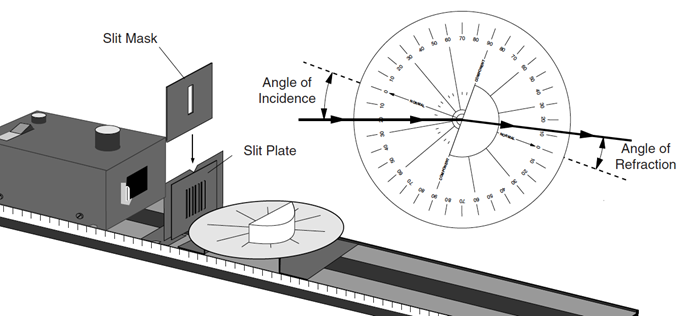
\includegraphics[width=1\linewidth]{images//figures/figure1.png}
    \caption{Visión completa del sistema}
    \label{fig:placeholder}
\end{figure}

\subsection{Procedimiento.}

\begin{itemize}
    \item Se instaló una fuente de luz en el banco óptico y, mediante una rendija (véase Figura~\ref{fig:fuente}), se formó un haz estrecho y bien colimado, orientado inicialmente sobre la marca de $0^\circ$ del disco graduado, garantizando la condición de incidencia normal.
    
    \item En el centro del soporte circular se posicionó cuidadosamente el medio de estudio (agua, acrílico o mezcla agua–café), de modo que para un ángulo de incidencia nulo el rayo emergente no presentara desviación. Esta verificación aseguró la correcta alineación del sistema óptico (Figura~\ref{fig:alineacion}).

    \item Posteriormente, se efectuaron mediciones consecutivas de los ángulos de incidencia $\theta_{1}$ y refracción $\theta_{2}$ para tres configuraciones distintas:
    \begin{enumerate}
        \item Lente semicilíndrica de acrílico (Figura~\ref{fig:montaje_acrilico}),
        \item Depósito semicircular con agua,
        \item Depósito semicircular con agua mezclada con café (Figura~\ref{fig:cafe}).
    \end{enumerate}

    \item En cada montaje, el disco graduado se giró en incrementos de $5^\circ$ o $10^\circ$ respecto de la normal, registrando los pares de valores $(\theta_{1}, \theta_{2})$ hasta que el rayo refractado dejara de ser visible o se alcanzara el ángulo crítico de reflexión total en el caso del acrílico.

    \item Finalmente, los datos obtenidos fueron tabulados y analizados aplicando la Ley de Snell, considerando la relación entre $\sin\theta_{1}$ y $\sin\theta_{2}$ para cada medio.
\end{itemize}

\begin{figure}[H]
    \centering
    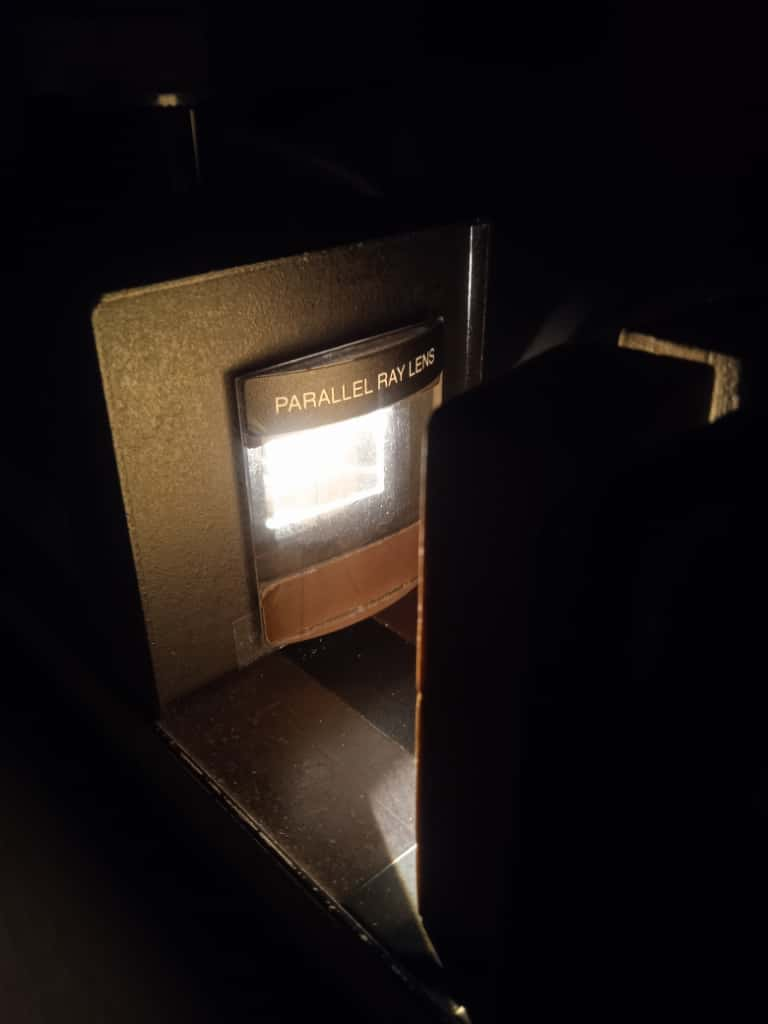
\includegraphics[width=0.7\linewidth]{images/photos/montaje_1.jpg}
    \caption{Fuente luminosa y rendija productora del haz colimado. Este montaje permitió generar un rayo fino y bien definido que incide sobre la marca de $0^\circ$ del disco.}
    \label{fig:fuente}
\end{figure}

\begin{figure}[H]
    \centering
    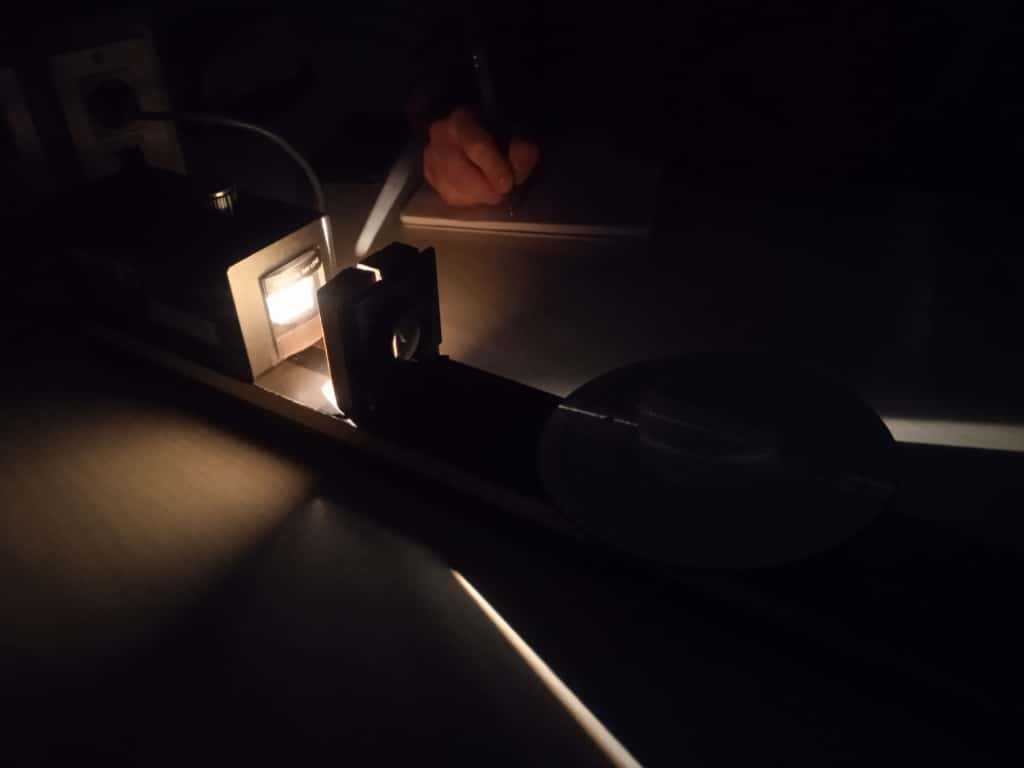
\includegraphics[width=0.7\linewidth]{images/photos/montaje_2.jpg}
    \caption{Alineación del haz incidente sobre el disco graduado. La correcta colocación del medio y del haz garantiza que, a incidencia normal, no exista desviación aparente.}
    \label{fig:alineacion}
\end{figure}

\begin{figure}[H]
    \centering
    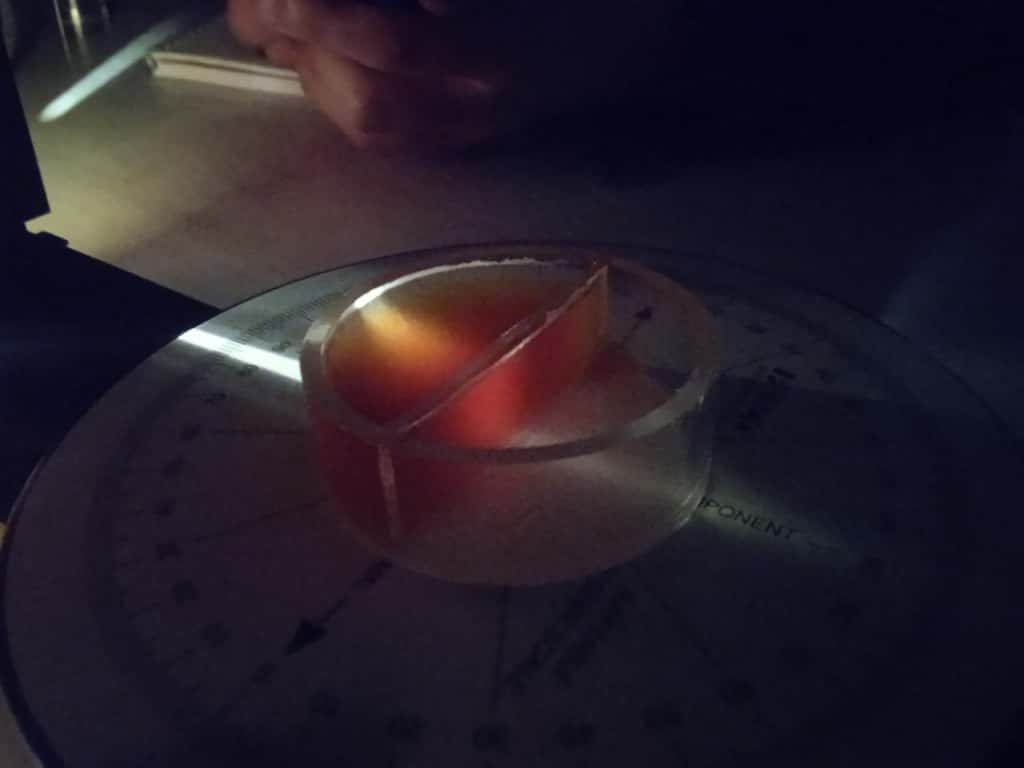
\includegraphics[width=0.7\linewidth]{images/photos/cafe_2.jpg}
    \caption{Refracción de la luz en la mezcla de agua con café. La turbidez del medio reduce la nitidez del rayo refractado y genera una mayor dispersión interna.}
    \label{fig:cafe}
\end{figure}

\begin{figure}[H]
    \centering
    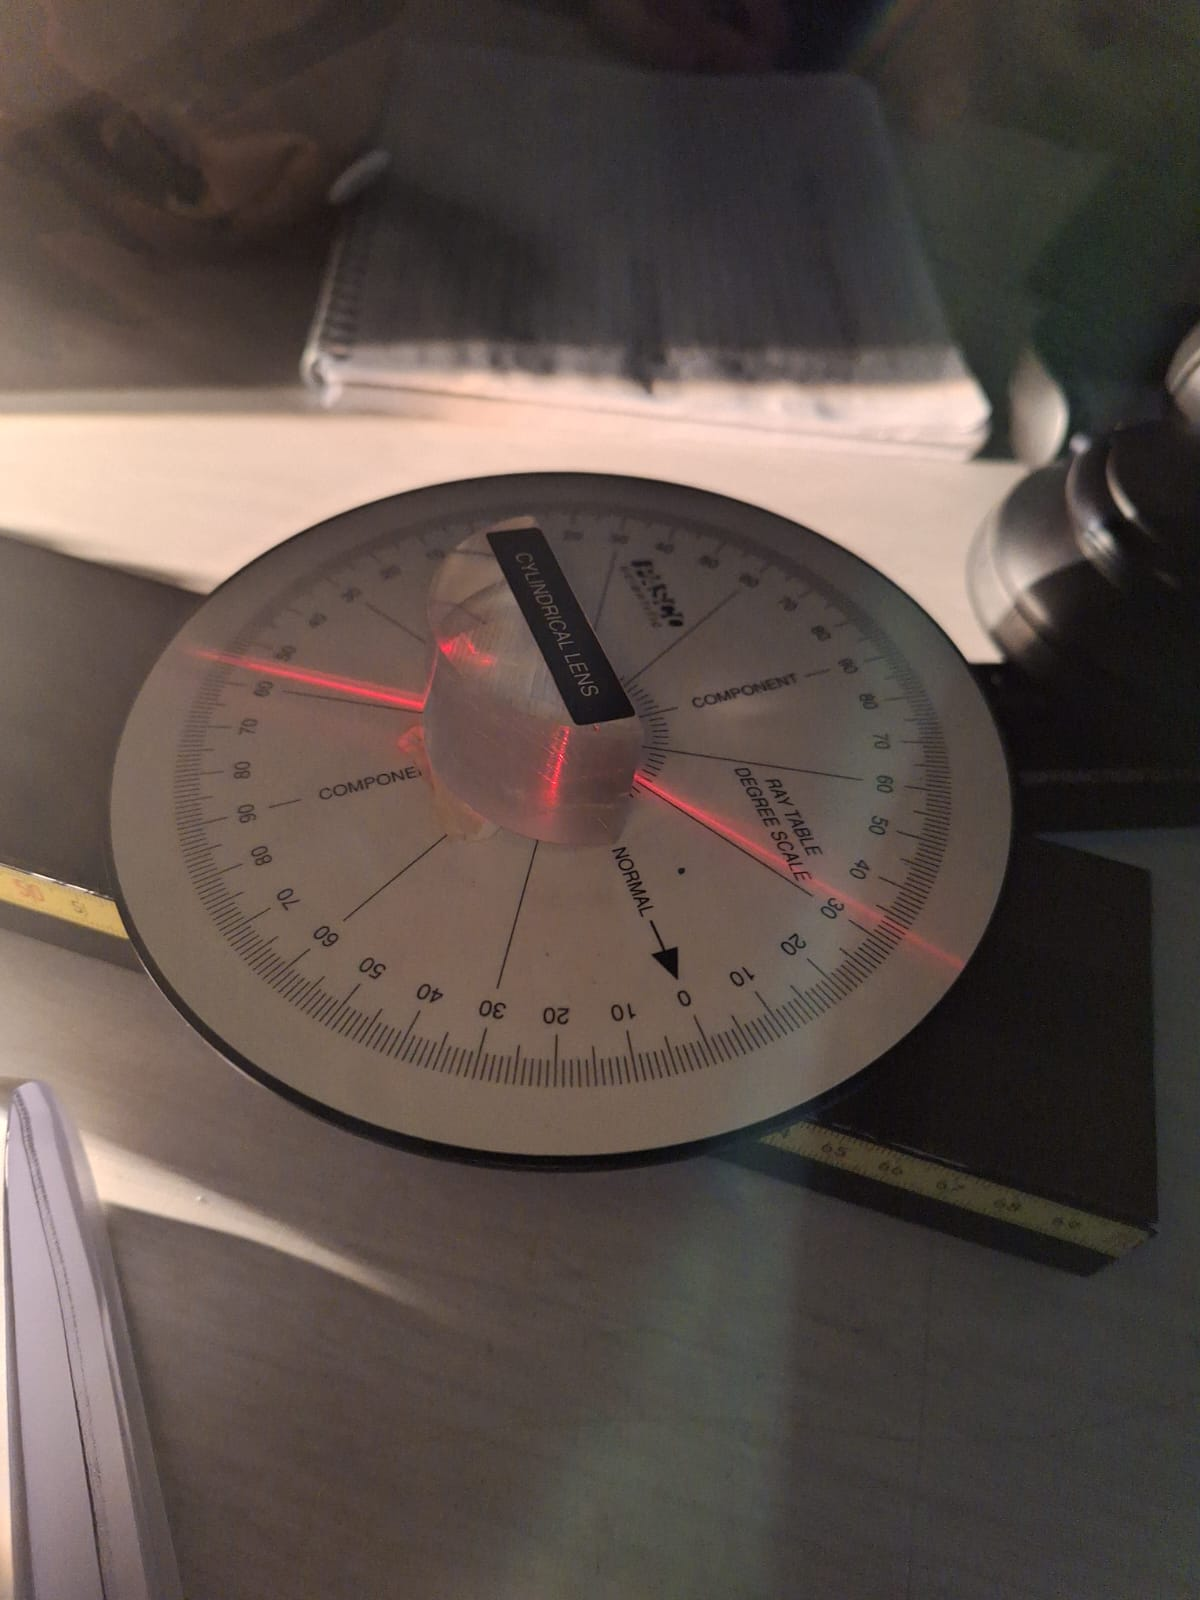
\includegraphics[width=0.7\linewidth]{images/photos/luz_monocromatica_refractada.jpg}
    \caption{Lente semicilíndrica de acrílico iluminada con luz monocromática. Se observa claramente el rayo refractado y la aparición del ángulo crítico de reflexión total.}
    \label{fig:montaje_acrilico}
\end{figure}


\section{Reporte de datos.}

Se registraron las mediciones de los ángulos de incidencia y refracción para distintos medios, 
organizadas según el sentido de propagación del haz. En cada caso se calcularon los valores 
de $\sin\theta_{1}$ y $\sin\theta_{2}$, que serán utilizados posteriormente para verificar 
la relación lineal predicha por la Ley de Snell.

\begin{itemize}
    \item \textbf{Agua:} incidencia por cara curva (Tabla~\ref{tab:agua_curva_plana}) y por cara plana (Tabla~\ref{tab:agua_plana_curva}).
    \item \textbf{Agua con café:} incidencia por cara curva (Tabla~\ref{tab:cafe_curva_plana}) y por cara plana (Tabla~\ref{tab:cafe_plana_curva}).
    \item \textbf{Acrílico:} determinación del ángulo crítico y verificación de la reflexión interna total (Tabla~\ref{tab:acrilico}).
\end{itemize}

\begin{table}[H]
\centering
\caption{Mediciones de los ángulos de incidencia y refracción en un depósito semicircular con \textbf{agua}. 
La luz incide desde el aire por la cara curva y emerge por la cara plana.}
\label{tab:agua_curva_plana}
\begin{tabular}{|c|c|c|c|}
\hline
$\theta_{1}$ (°) & $\sin\theta_{1}$ & $\theta_{2}$ (°) & $\sin\theta_{2}$ \\ \hline
10 & 0,17 & 15 & 0,26 \\
20 & 0,34 & 39 & 0,63 \\
30 & 0,50 & 44 & 0,69 \\
40 & 0,64 & 64 & 0,90 \\
66 & 0,91 & 46 & 0,72 \\ \hline
\end{tabular}
\end{table}

\begin{table}[H]
\centering
\caption{Mediciones de incidencia y refracción en un depósito semicircular con \textbf{agua}. 
La luz incide desde el aire por la cara plana y emerge por la cara curva.}
\label{tab:agua_plana_curva}
\begin{tabular}{|c|c|c|c|}
\hline
$\theta_{1}$ (°) & $\sin\theta_{1}$ & $\theta_{2}$ (°) & $\sin\theta_{2}$ \\ \hline
0 & 0,00 & 0 & 0,00 \\
10 & 0,17 & 16 & 0,28 \\
20 & 0,34 & 23 & 0,39 \\
30 & 0,50 & 30 & 0,50 \\
40 & 0,64 & 36 & 0,59 \\
50 & 0,77 & 41 & 0,66 \\
60 & 0,87 & 45 & 0,71 \\
70 & 0,94 & 50 & 0,77 \\
80 & 0,98 & --- & --- \\
90 & 1,00 & --- & --- \\ \hline
\end{tabular}
\end{table}

\begin{table}[H]
\centering
\caption{Mediciones de incidencia y refracción en un depósito semicircular con \textbf{agua mezclada con café}. 
La luz incide desde el aire por la cara curva y emerge por la cara plana.}
\label{tab:cafe_curva_plana}
\begin{tabular}{|c|c|c|c|}
\hline
$\theta_{1}$ (°) & $\sin\theta_{1}$ & $\theta_{2}$ (°) & $\sin\theta_{2}$ \\ \hline
7 & 0,12 & 10 & 0,17 \\
10 & 0,17 & 15 & 0,26 \\
20 & 0,34 & 30 & 0,50 \\
30 & 0,50 & 45 & 0,71 \\
40 & 0,64 & 62 & 0,88 \\ \hline
\end{tabular}
\end{table}

\begin{table}[H]
\centering
\caption{Mediciones de incidencia y refracción en un depósito semicircular con \textbf{agua con café}. 
La luz incide desde el aire por la cara plana y emerge por la cara curva.}
\label{tab:cafe_plana_curva}
\begin{tabular}{|c|c|c|c|}
\hline
$\theta_{1}$ (°) & $\sin\theta_{1}$ & $\theta_{2}$ (°) & $\sin\theta_{2}$ \\ \hline
10 & 0,17 & 6 & 0,10 \\
20 & 0,34 & 13 & 0,22 \\
30 & 0,50 & 21 & 0,36 \\
40 & 0,64 & 28 & 0,47 \\
50 & 0,77 & 33 & 0,54 \\
60 & 0,87 & 39 & 0,63 \\
70 & 0,94 & 43 & 0,68 \\
80 & 0,98 & --- & --- \\
90 & 1,00 & --- & --- \\ \hline
\end{tabular}
\end{table}

\begin{table}[H]
\centering
\caption{Determinación experimental del ángulo crítico en una lente semicircular de \textbf{acrílico}. 
Se observa la refracción hasta el límite de reflexión total interna.}
\label{tab:acrilico}
\begin{tabular}{|c|c|c|c|}
\hline
$\theta_{1}$ (°) & $\sin\theta_{1}$ & $\theta_{2}$ (°) & $\sin\theta_{2}$ \\ \hline
0 & 0,00 & 0 & 0,00 \\
5 & 0,09 & 7 & 0,12 \\
10 & 0,17 & 16 & 0,26 \\
15 & 0,26 & 22 & 0,37 \\
20 & 0,34 & 30 & 0,50 \\
25 & 0,43 & 38 & 0,62 \\
30 & 0,50 & 46 & 0,72 \\
35 & 0,57 & 56 & 0,83 \\
40 & 0,64 & 70 & 0,94 \\
45 & 0,71 & --- & --- \\ \hline
\end{tabular}
\end{table}

\section{Análisis de datos.}

\subsection{Representación gráfica de la Ley de Snell.}

A partir de los datos experimentales de cada medio y orientación de la lente semicircular, 
se construyeron los pares $(\sin\theta_{1},\, \sin\theta_{2})$ con el fin de verificar 
la linealidad prevista por la Ley de Snell. En cada gráfico se muestra el ajuste lineal 
obtenido y su ecuación correspondiente. 

\begin{itemize}
    \item Para la refracción del \textbf{aire hacia el agua con café (cara plana)}, véase la Figura~\ref{fig:aire_cafe_plana}.
    \item Para la refracción del \textbf{aire hacia el agua con café (cara curva)}, véase la Figura~\ref{fig:aire_cafe_curva}.
    \item Para la refracción del \textbf{agua hacia el aire (cara plana)}, véase la Figura~\ref{fig:agua_aire_plana}.
    \item Para la refracción del \textbf{agua hacia el aire (cara curva)}, véase la Figura~\ref{fig:agua_aire_curva}.
    \item Para la refracción del \textbf{agua con café} (ajuste global, combinando ambas caras), véase la Figura~\ref{fig:agua_cafe_global}.
    \item Para la refracción y \textbf{reflexión total interna en acrílico}, véase la Figura~\ref{fig:acrilico_ajuste}.
\end{itemize}

\begin{figure}[H]
    \centering
    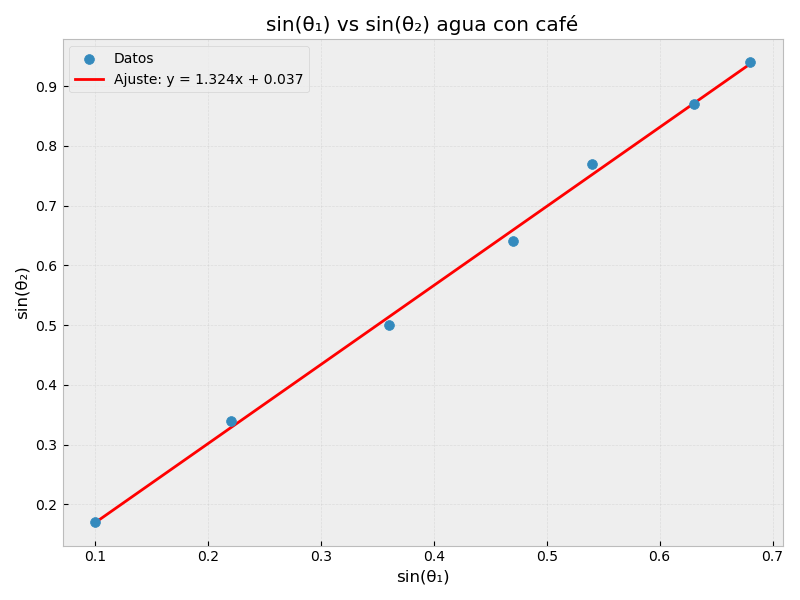
\includegraphics[width=\linewidth]{images/plots/1.png}
    \caption{Relación entre $\sin\theta_{1}$ y $\sin\theta_{2}$ para la refracción del \textbf{aire hacia el agua con café por la cara plana}. 
    El ajuste lineal $y = 1.324x + 0.037$ muestra un comportamiento cercano a la proporcionalidad esperada, 
    indicando un índice de refracción efectivo de $n \approx 1/1.324 \simeq 0.76$, 
    cuya inversión debe corregirse considerando el sentido óptico (medio de incidencia).}
    \label{fig:aire_cafe_plana}
\end{figure}

\begin{figure}[H]
    \centering
    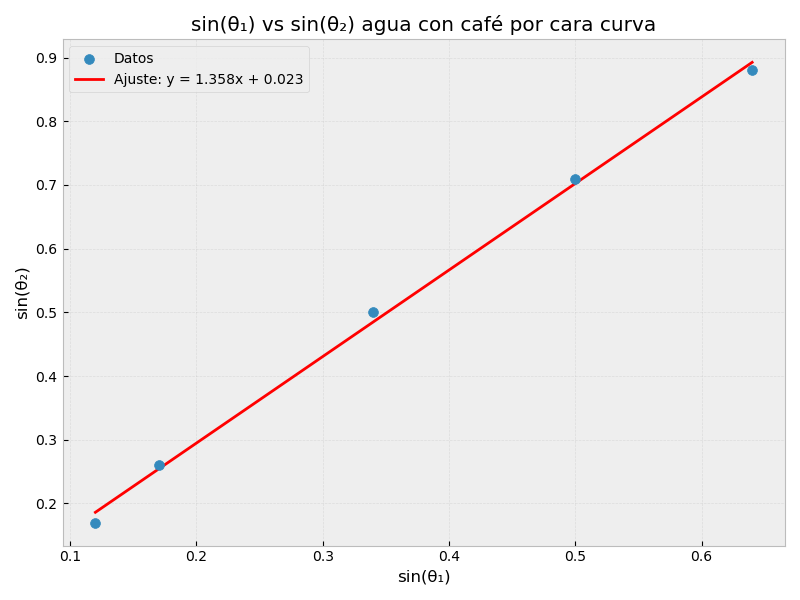
\includegraphics[width=\linewidth]{images/plots/4.png}
    \caption{Relación entre $\sin\theta_{1}$ y $\sin\theta_{2}$ para la refracción del \textbf{aire hacia el agua con café por la cara curva}. 
    El ajuste $y = 1.358x + 0.023$ es similar al caso anterior, con pendiente ligeramente mayor, 
    atribuible a diferencias en la alineación y curvatura de la superficie.}
    \label{fig:aire_cafe_curva}
\end{figure}

\begin{figure}[H]
    \centering
    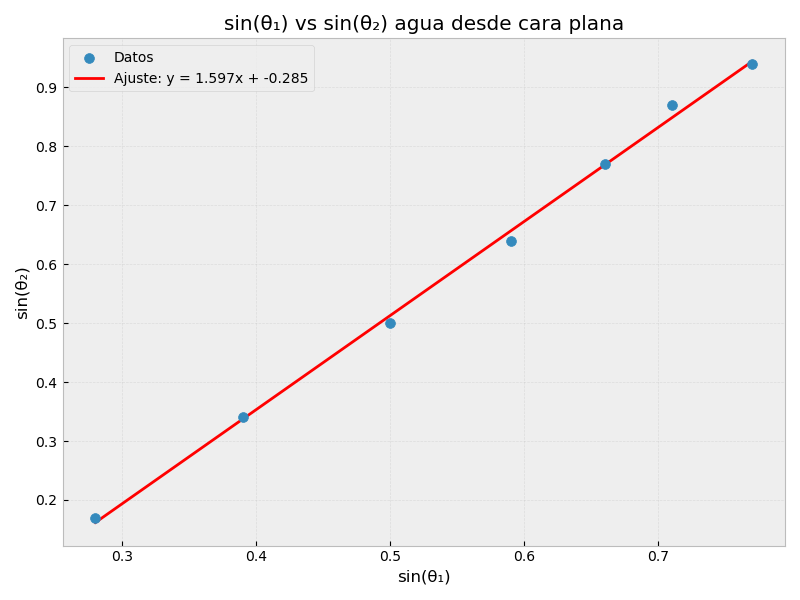
\includegraphics[width=\linewidth]{images/plots/3.png}
    \caption{Relación entre $\sin\theta_{1}$ y $\sin\theta_{2}$ para la refracción del \textbf{agua hacia el aire por la cara plana}. 
    La pendiente $m=1.597$ corresponde al paso del medio denso al menos denso, coherente con un ángulo crítico de $\theta_c \approx 39^\circ$.}
    \label{fig:agua_aire_plana}
\end{figure}

\begin{figure}[H]
    \centering
    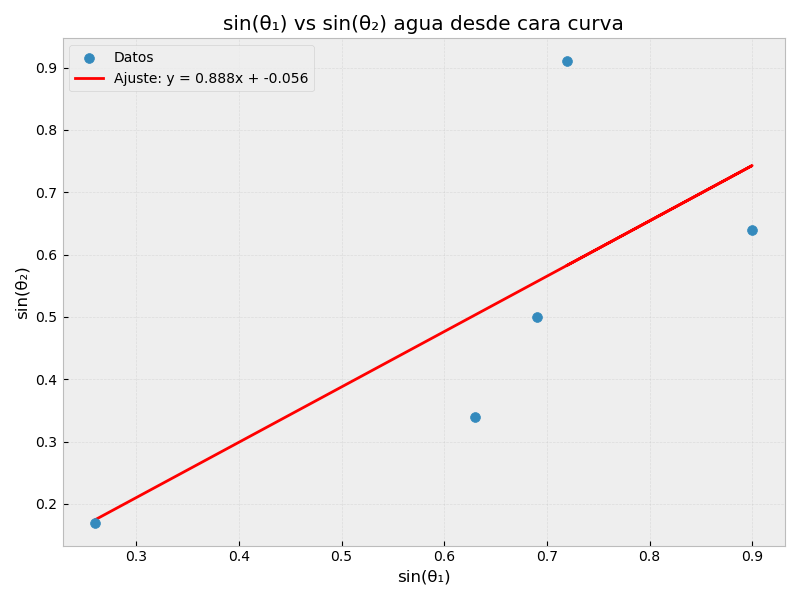
\includegraphics[width=\linewidth]{images/plots/2.png}
    \caption{Relación entre $\sin\theta_{1}$ y $\sin\theta_{2}$ para la refracción del \textbf{agua hacia el aire por la cara curva}. 
    La dispersión de los puntos y la pendiente $m=0.888$ reflejan mayor error experimental, probablemente por la dificultad 
    de definir con precisión el ángulo refractado en la interfaz curva.}
    \label{fig:agua_aire_curva}
\end{figure}

\begin{figure}[H]
    \centering
    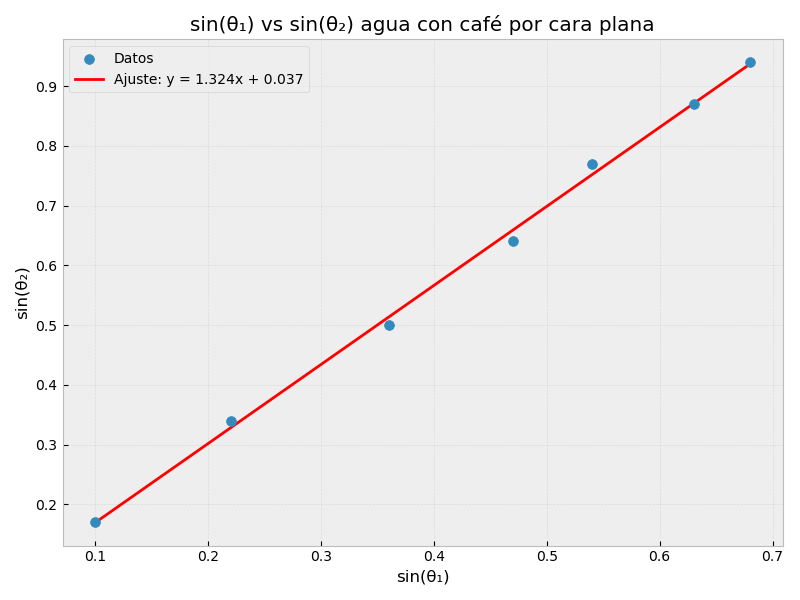
\includegraphics[width=\linewidth]{images/plots/5.png}
    \caption{Refracción del \textbf{agua con café} considerando el conjunto de mediciones experimentales. 
    La relación lineal $y = 1.324x + 0.037$ muestra consistencia con las determinaciones individuales, 
    validando la tendencia global observada.}
    \label{fig:agua_cafe_global}
\end{figure}

\begin{figure}[H]
    \centering
    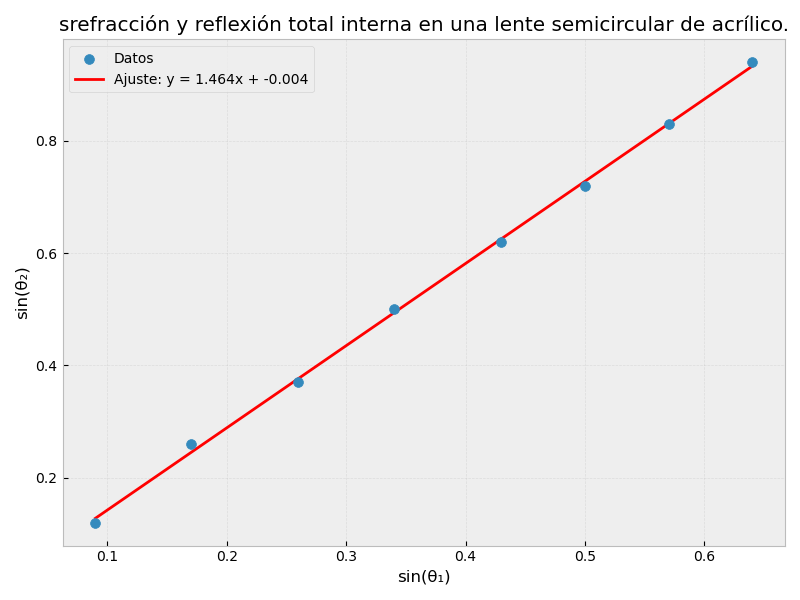
\includegraphics[width=\linewidth]{images/plots/6.png}
    \caption{Refracción y \textbf{reflexión total interna} en una lente semicircular de acrílico. 
    La pendiente $m=1.464$ del ajuste $y = 1.464x - 0.004$ es coherente con el valor teórico del índice de refracción del acrílico 
    ($n_{\text{acrílico}} \approx 1.49$), confirmando la validez de la Ley de Snell y del método experimental.}
    \label{fig:acrilico_ajuste}
\end{figure}

\subsection{Comparación entre los distintos medios.}

Al comparar los resultados obtenidos para los tres medios estudiados (acrílico, agua y agua con café), se observan diferencias significativas en su comportamiento óptico, asociadas principalmente a su homogeneidad y transparencia.

\begin{itemize}
    \item \textbf{Acrílico:} Medio homogéneo y transparente, mostró una relación lineal clara entre $\sin \theta_1$ y $\sin \theta_2$, con una pendiente que permitió estimar un índice de refracción cercano a 1,47. Además, fue posible identificar claramente el ángulo crítico ($\theta_c \approx 43^\circ$), lo que confirma su mayor densidad óptica.
    
    \item \textbf{Agua:} También transparente y homogénea, presentó un comportamiento lineal consistente con la Ley de Snell, con un índice de refracción experimental próximo a 1,33. No se alcanzó el ángulo crítico dentro del rango medido, como era esperable.
    
    \item \textbf{Agua con café:} La presencia de partículas en suspensión introdujo dispersión y atenuación del haz, lo que aumentó la incertidumbre en la medición de $\theta_2$. Aunque la relación $\sin \theta_1$ vs $\sin \theta_2$ se mantuvo aproximadamente lineal, la pendiente varió ligeramente en comparación con el agua pura, sugiriendo un pequeño aumento en el índice de refracción debido a la concentración de sólidos disueltos.
\end{itemize}

Estas diferencias resaltan la influencia de la composición y pureza del medio en la propagación de la luz, validando la Ley de Snell en medios ideales y mostrando desviaciones en medios con inhomogeneidades.


\subsection{Ensanchamiento del haz luminoso.}

Durante el experimento se observó que el haz luminoso tendía a ensancharse al emerger del medio, especialmente en configuraciones con incidencia oblicua y en medios no completamente transparentes como el agua con café.

Este fenómeno puede atribuirse a dos factores principales:

\begin{enumerate}
    \item \textbf{Refracción en interfaces curvas:} Al ingresar o salir del semicilindro, la geometría curva de la interfase produce que distintos rayos del haz incidan con ángulos ligeramente diferentes, generando un abanico de direcciones emergentes.
    
    \item \textbf{Dispersión en medios turbios:} En el caso del agua con café, las partículas en suspensión dispersan la luz en múltiples direcciones, lo que ensancha el haz y reduce su intensidad. Este efecto es más notable a mayores ángulos de incidencia, donde la trayectoria dentro del medio es más larga.
\end{enumerate}

El ensanchamiento del haz no invalida la Ley de Snell, pero sí introduce limitaciones prácticas en la precisión de las mediciones, especialmente en medios no homogéneos.


\section{Discusión:}

Obtuvimos las siguientes mediciones:
\begin{align*}
    n_1 &=1.324\\
    n_2 &= 0.888 \\ 
    n_3 &= 1.597 \\ 
    n_4 &= 1.358 \\
    n_6 &= 1.464
\end{align*}
Cada uno corresponde a su gráfico y tabla correspondiente. Con el propósito de enumerar, ignoraremos su procedencia, de momento.

En los experimentos obtuvimos reflexión total interna, es claro que $n>1$, pues aquí consideramos como referencia el rayo dentro del vidrio/acrílico. En estos casos, encontramos que:
\begin{align*}
    \theta_{1,c}&\approx 46.6^{\circ}\\
    \theta_{2,c}&\approx \text{undefined}\\
    \theta_{3,c}&\approx 40.0\\
    \theta_{4,c}&\approx46.0^{\circ}\\
    \theta_{5,c}&\approx 43.2^{\circ}
\end{align*}
donde usamos la recta de mínimos cuadrados, interceptamos en $y=1$ y luego calculamos
\begin{align*}
    \theta^{\circ}&=\frac{\arcsin(x)}{2\pi}360\\
    x&=\frac{1-b}{n}
\end{align*}
La discrepancia de $n_2$ corresponde a la grán desviación que hay entre cada dato ($R^2\approx 0.5$). Debido a esto, no podemos obtener conclusiones de esta gráfica.
\section{Conclusiones.}

%%%%%%%%%%%%%%%%%%%%%%%%%%%%%%%%%%%% DEEPSEEK CONCLUSION &&&&&&&&&&&&&&&&&&&&&&&&&&&&&&&&

\begin{itemize}
    \item Se verificó experimentalmente la Ley de Snell para todos los medios estudiados (acrílico, agua y agua con café), observándose una relación lineal consistente entre $\sin\theta_1$ y $\sin\theta_2$, con coeficientes de determinación cercanos a 1 en la mayoría de los casos, aunque se registró mayor dispersión en los datos para el agua con café debido a efectos de atenuación y dispersión lumínica.

    \item Se determinó el índice de refracción para cada medio, obteniéndose valores consistentes con los reportados en la literatura:
    \begin{itemize}
        \item $n_{\text{acrílico}} \approx 1,47$
        \item $n_{\text{agua}} \approx 1,33$ 
        \item $n_{\text{agua con café}} \approx 1,36$ (ligeramente superior al agua pura, atribuible a la presencia de partículas en suspensión)
    \end{itemize}

    \item Se identificó el ángulo crítico de reflexión total interna en el acrílico ($\theta_c \approx 43^\circ$), validando cuantitativamente el modelo teórico y confirmando que este fenómeno solo ocurre cuando la luz pasa de un medio más denso a uno menos denso.

    \item Se observó que la turbidez del medio (agua con café) introduce dispersión y ensanchamiento del haz, lo que aumenta la incertidumbre en la medición de $\theta_2$, constituyendo una limitación práctica para la precisión de las mediciones, aunque sin invalidar los principios ópticos fundamentales.

    \item El montaje experimental con semicilindros resultó adecuado para el estudio cuantitativo de la refracción, permitiendo minimizar errores de alineación y facilitar la medición directa de ángulos.

    \item Como recomendación, para futuros experimentos se sugiere el uso de sensores de posición o videoanálisis para reducir la incertidumbre en la medición de ángulos, especialmente en medios semitransparentes donde el haz se atenúa y dispersa.
\end{itemize}

\newpage{}
\onecolumn{}
\printbibliography

\end{document}
